\section{Задание}

\begin{figure}[H]
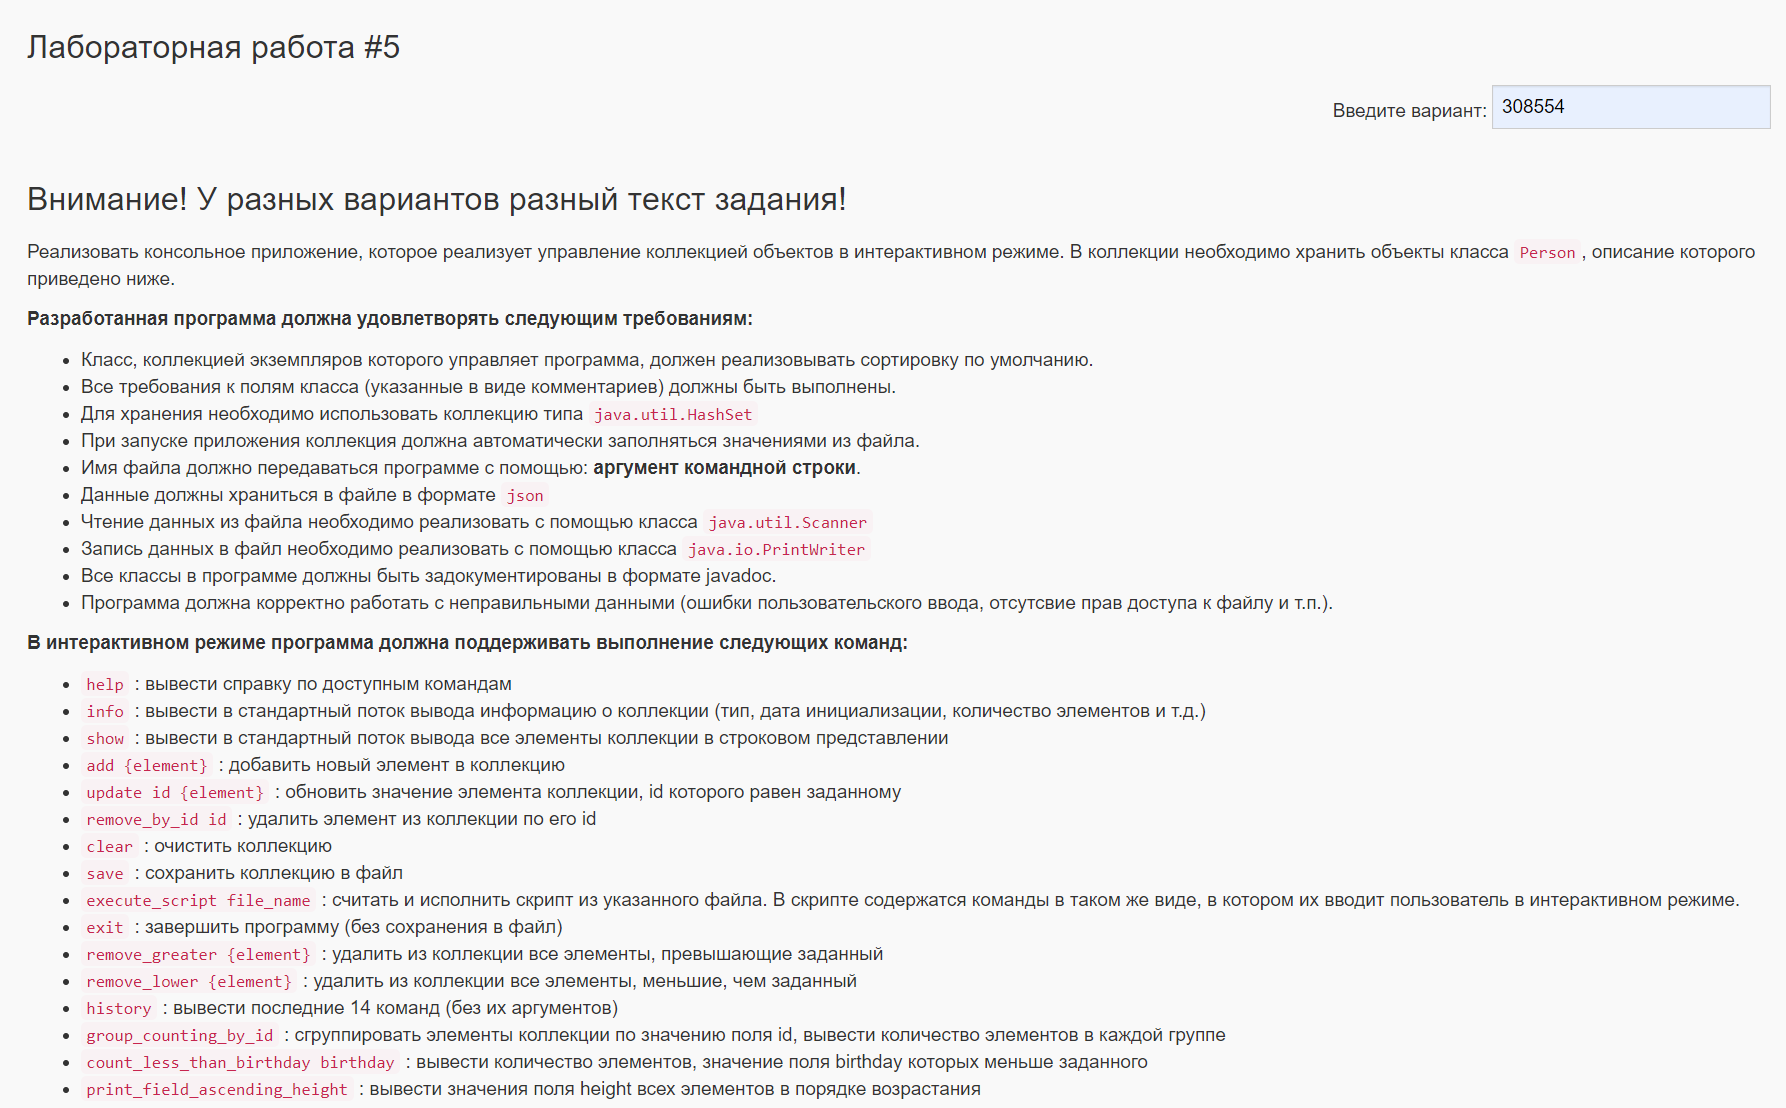
\includegraphics[width=\textwidth,height=\textheight,keepaspectratio]{img/task1}
\label{pic:task1}
\end{figure}

\begin{figure}[H]

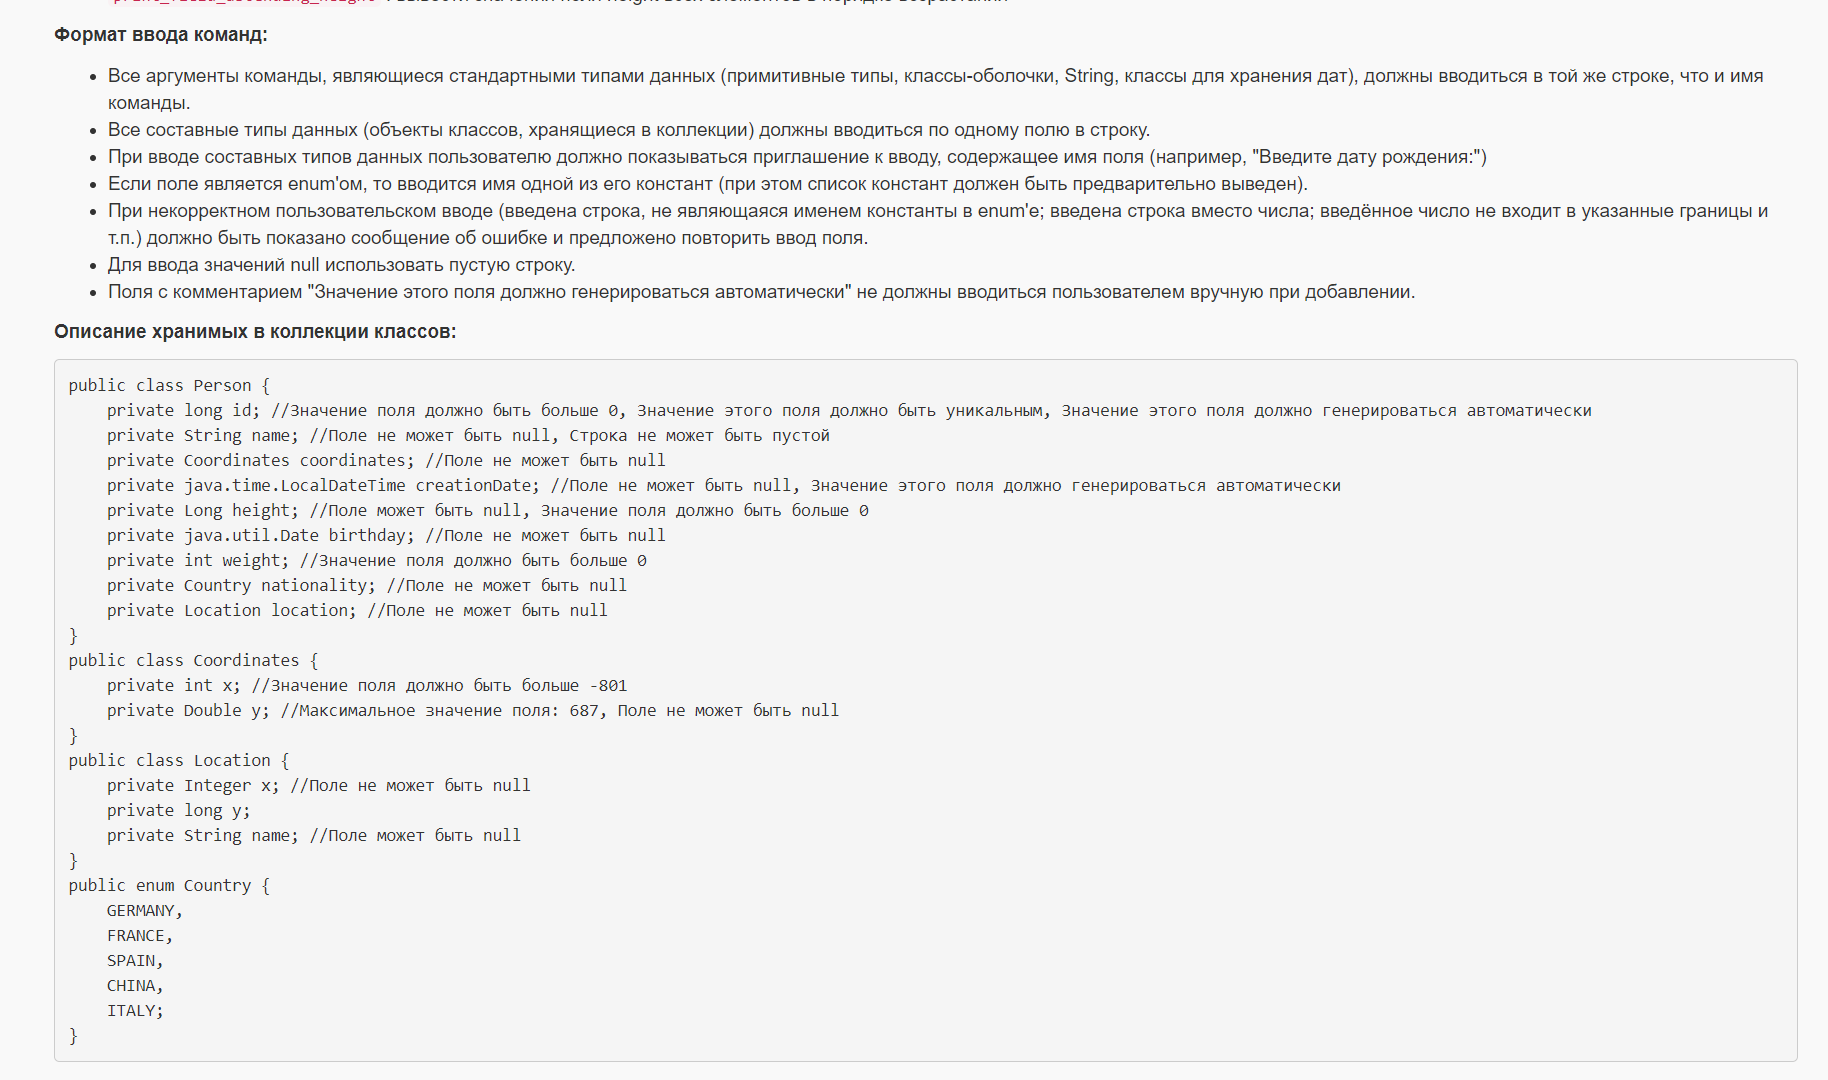
\includegraphics[width=\textwidth,height=\textheight,keepaspectratio]{img/task2}
\label{pic:task2}
\end{figure}

\newpage
\section{Код и Диаграмм}
\textbf{Исходный код доступен по ссылке или QR-коду:}\\
\\     
\underline{$https://github.com/ndwannafly/Programming-Lab-2nd-Semester/tree/main/LAB_5$}\\


\begin{figure}[H]

\includegraphics[scale=0.8]{img/SourceCode}
\label{pic:SourceCode}
\end{figure}

\underline{$https://github.com/ndwannafly/Programming-Lab-2nd-Semester/blob/main/LAB_5/отчёт/diagram.png$}\\


\begin{figure}[H]

\includegraphics[scale=0.8]{img/QRDiagram}
\label{pic:QRDiagram}
\end{figure}

\section{Вывод}
В ходе этой лабораторной работы мы знаем о Collection Java Framework, а также как использовать Javadoc, работать с потоками, файлами, интерфейсами Comparable и Comparator. Кроме того, мы знаем, как применять шаблоны проектирования для соблюдения принципов SOLID.